\chapter{Multi-scale modelling of dry granular flows}

\ifpdf
    \graphicspath{{Chapter4/figs/raster/}{Chapter4/figs/pdf/}{Chapter4/figs/}}
\else
    \graphicspath{{Chapter4/figs/vector/}{Chapter4/figs/}}
\fi

\section{Introduction}

The dynamics of a homogeneous granular flow involve at least three distinct 
scales: the \textit{microscopic scale}, which 
is characterised by the contact between grains, the \textit{meso-scale} that 
represents micro-structural effects such as grain rearrangement, and the 
\textit{macroscopic scale}, where geometric correlations can be observed (see 
Figure~\ref{fig:multiscale}). Conventionally, granular flows are modelled as a 
continuum because they exhibit many collective phenomena. However, on a grain 
scale, the granular materials exhibit complex solid-like and/or fluid-like 
behaviour.Recent studies, however, suggest that a continuum law may be unable 
to capture the effect of inhomogeneities at the grain scale level, such as 
orientation of force chains, which are micro-structural effects. Discrete 
element methods (DEM) are capable of simulating these micro-structural effects, 
however they are computationally expensive. In the present study, a multi-scale 
approach is adopted, using both DEM and continuum techniques, to better 
understand the rheology of granular flows and the limitations of continuum 
models.

\begin{figure}[tbhp]
\centering
\includegraphics[width=0.95\textwidth]{multiscale}
\caption{Multi-scale modelling of granular materials}
\label{fig:multiscale}
\end{figure}

\section{Granular column collapse}

The collapse of a granular column on a horizontal surface is a simple case of 
granular flow, however a proper model that describes the flow dynamics is still
lacking. Granular flow is modelled as a frictional dissipation process in 
continuum mechanics but studies showing the lack of influence of inter-particle 
friction on the energy dissipation and spreading dynamics is surprising. 
In the present study, the generalised interpolation material point method 
(GIMPM), a hybrid Eulerian -- Lagrangian approach, is implemented with 
Mohr-Coloumb failure criterion to describe the continuum behaviour of quasi-two 
dimensional collapse of granular columns. The granular column collapse is also 
simulated using DEM to understand the micro-mechanics of the flow.

~\citet{Lajeunesse2005} performed axis-symmetric and plane strain tests on 
granular column collapse. Granular materials when released suddenly on a 
horizontal surface exhibit transient flow. The mechanism of flow initiation, 
spreading dynamics and energy dissipation are studied. The experimental 
configuration used by~\citet{Lajeunesse2005} is shown in Figure~\ref{fig:exp}. 
Granular material of mass `\textit{M}' was poured into a container to form a 
rectangular heap of length `${L}_{\textit{i}}$', height `${H}_{\textit{i}}$' 
and thickness `\textit{W}'. The internal friction angle and the wall friction 
between the wall and the glass beads measured by ~\citet{Lajeunesse2005} are 
listed in Table~\ref{table:mat_prop}. The gate was then quickly removed to 
release the granular mass that spreads in the horizontal channel until it comes 
to rest. The final run-out distance `${L}_{\textit{f}}$' and the collapsed 
height `$H_{\textit{f}}$' were measured. The run-out distance and collapse 
height were found to exhibit power law relation with the initial aspect ratio 
`\textit{a}' $(=H_{\textit{i}}/L_{\textit{i}})$ of the column. 

\begin{figure}[tbhp]
\centering
\includegraphics[width=0.85\textwidth]{experiment_setup}
\caption{Schematic of experimental configuration for 2-D collapse in a 
rectangular channel,~\citep{Lajeunesse2005}}
\label{fig:exp}
\end{figure}

\begin{table}[tbhp]
\caption{Material properties of glass ballotini,~\citep{Lajeunesse2005}}
\label{table:mat_prop}
\centering
\begin{tabular}{ll}
\toprule
\textbf{Parameter} & \textbf{Value} \\ \midrule
Mean diameter & 1.15 mm \\
Repose angle & 22$\pm 0.5^{o} $\\
Avalanche angle & 27.4$\pm 0.5^{o} $\\
Wall friction angle & 24.8$\pm 0.2^{o} $\\
\bottomrule
\end{tabular}
\end{table}

\begin{figure}[tbhp]
\centering
\includegraphics[width=\textwidth]{a04tc}
\caption{Velocity profile of a granular column collapse ($`a' = 0.4 \& 
t=\tau_c$)}
\label{fig:a04tc}
\end{figure}

\begin{figure}[tbhp]
\centering
\includegraphics[width=0.45\textwidth]{simple_shear}
\caption{Shear test periodic boundary condition}
\label{fig:shear}
\end{figure}

\begin{figure}[tbhp]
\centering
\includegraphics[width=\textwidth]{a04f}
\caption{Velocity profile of a granular column collapse ($`a' = 0.4 \& 
t=3\times\tau_c$)}
\label{fig:a04f}
\end{figure}

\begin{figure}[tbhp]
\centering
\includegraphics[width=\textwidth]{a6tc}
\caption{Velocity profile of a granular column collapse ($`a' = 6 \& 
t=\tau_c$)}
\label{fig:a6tc}
\end{figure}

\begin{figure}[tbhp]
\centering
\includegraphics[width=\textwidth]{a6f}
\caption{Velocity profile of a granular column collapse ($`a' = 6 \& 
t=3\times\tau_c$)}
\label{fig:a6f}
\end{figure}

%\begin{landscape}
%\centering
\begin{figure}[tbhp]
\centering
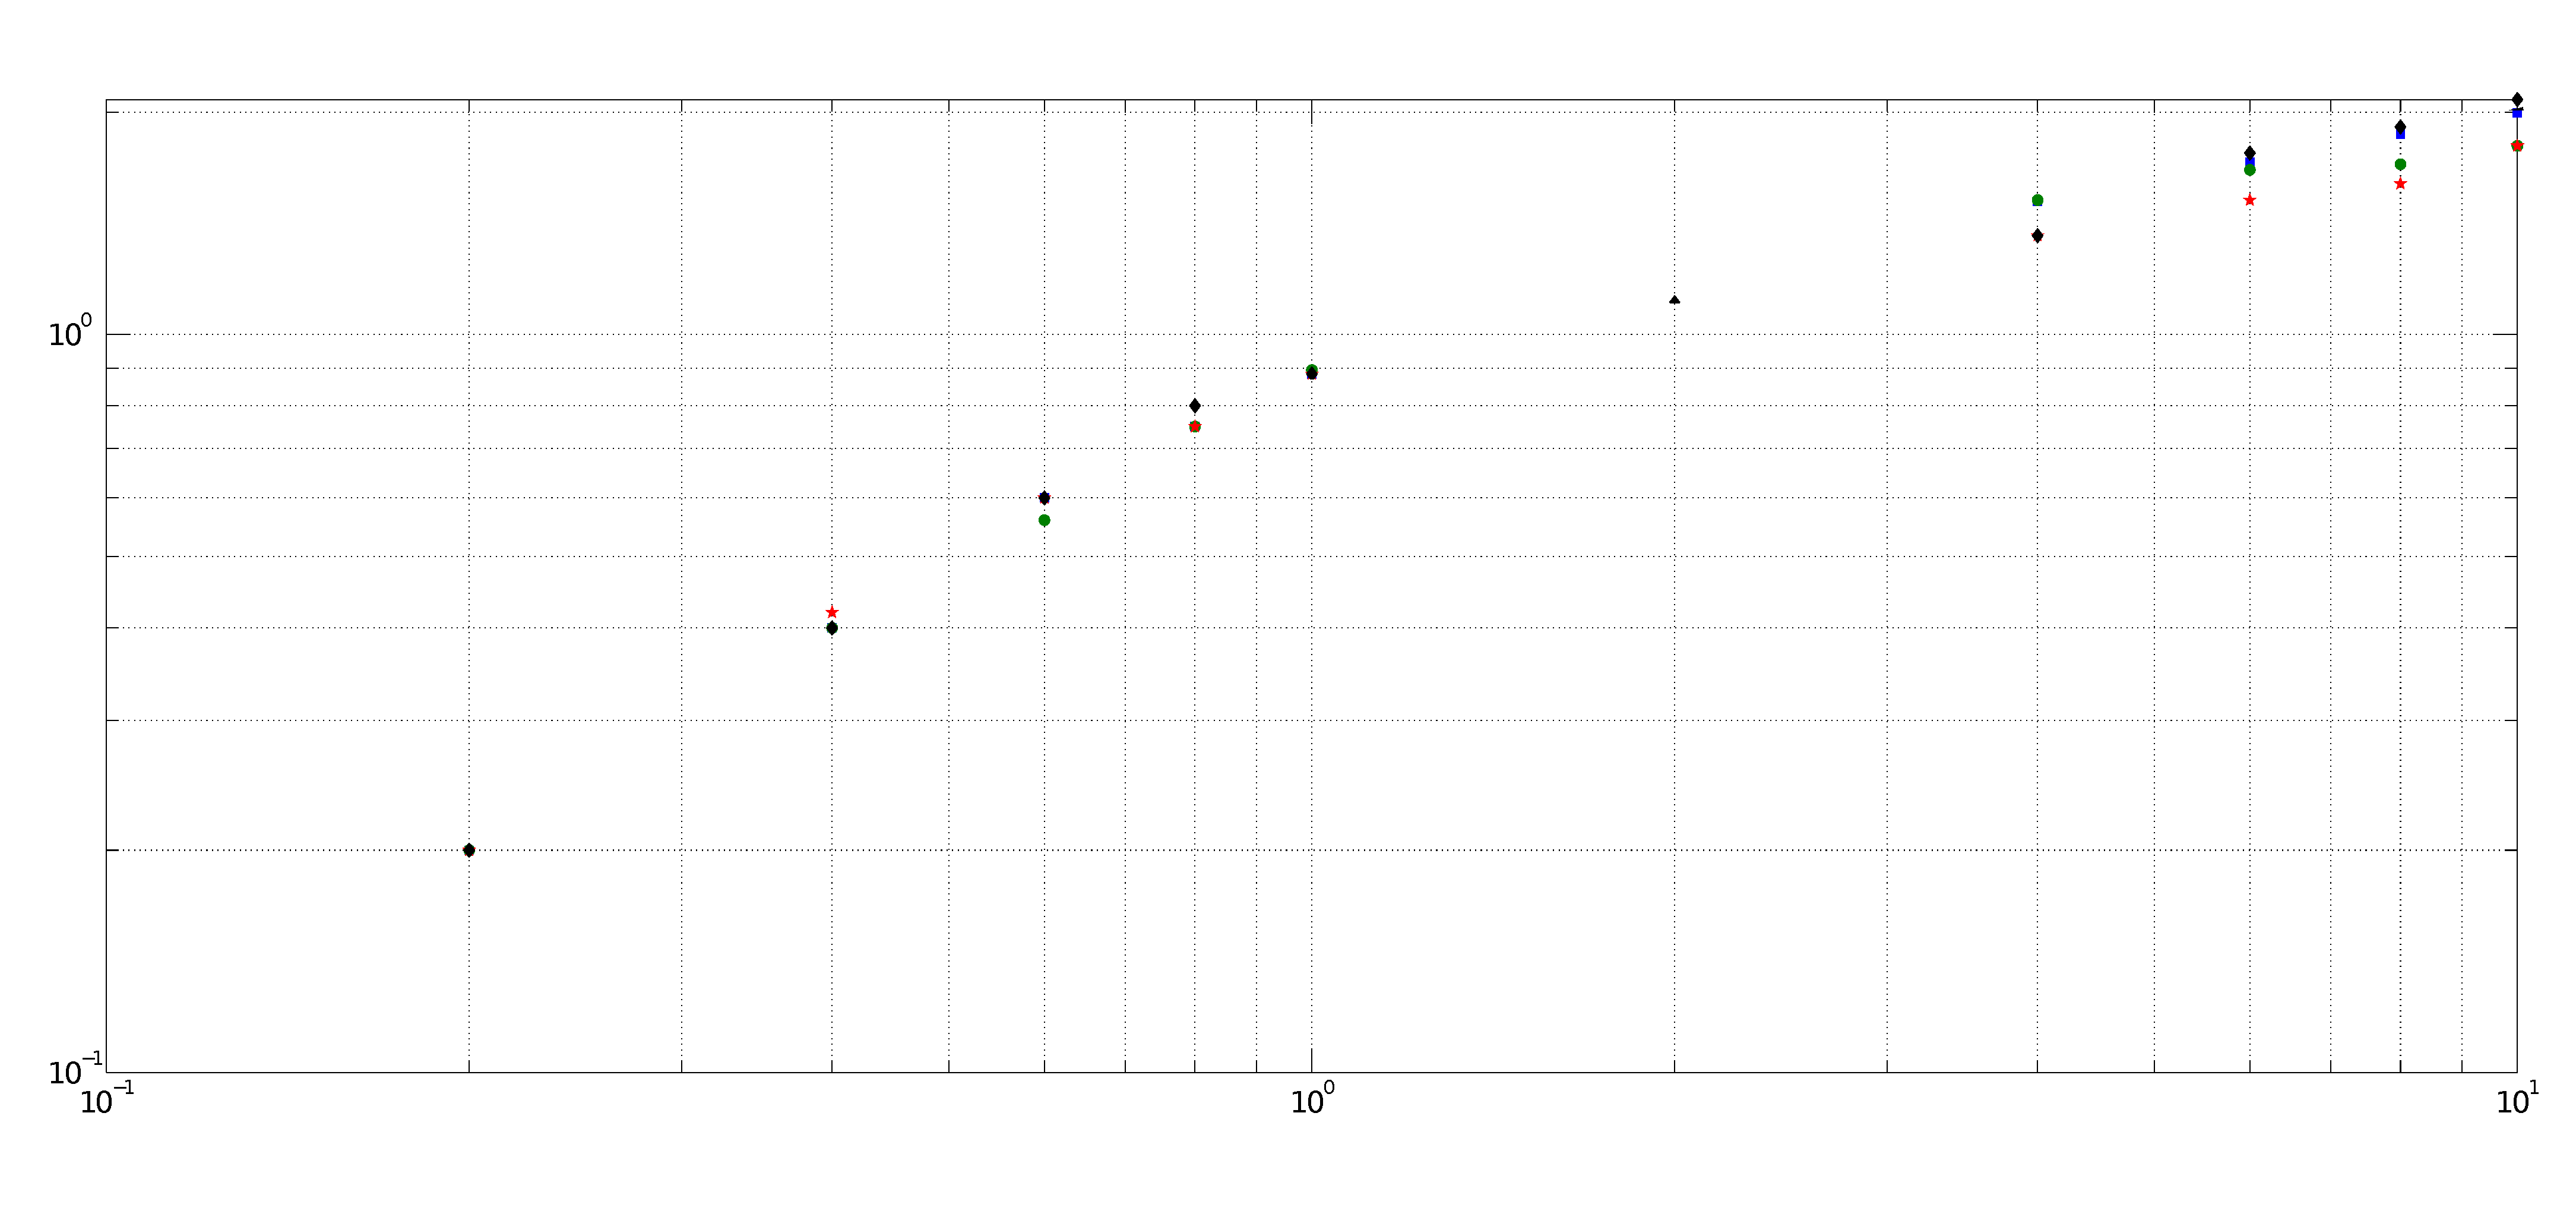
\includegraphics[width=\textwidth]{height}
\caption{Final collapse height for columns with different initial aspect ratio}
\label{fig:height}
\end{figure}
%\end{landscape}

\begin{figure}[tbhp]
\centering
\includegraphics[width=\textwidth]{flowa04}
\caption{Flow evolution of a column with $`a'=0.4$}
\label{fig:flowa04}
\end{figure}

\begin{figure}[tbhp]
\centering
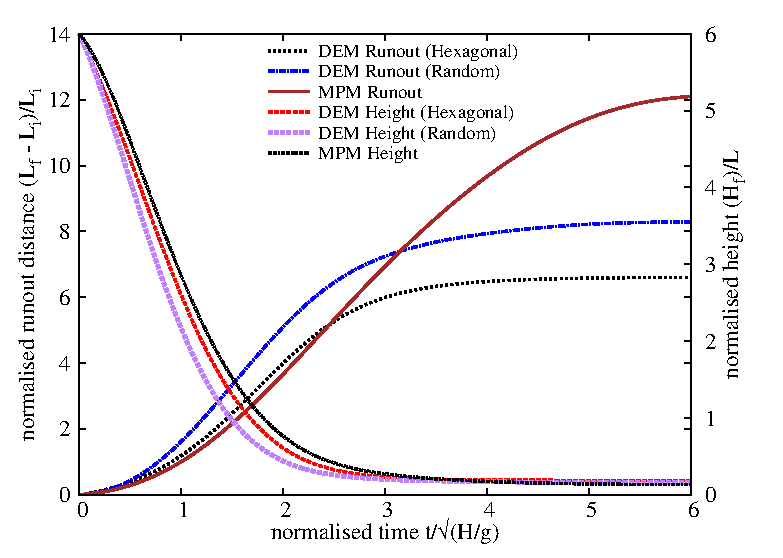
\includegraphics[width=\textwidth]{flowa6}
\caption{Flow evolution of a column with $`a'=6$}
\label{fig:flowa6}
\end{figure}
